\documentclass[12pt,a4paper]{article}
\usepackage[T2A]{fontenc}
\usepackage[utf8]{inputenc}
\usepackage[russian]{babel}

\usepackage{graphicx}
\graphicspath{{img/}}
\DeclareGraphicsExtensions{.png}

\usepackage{float}
\usepackage{hyperref}
\usepackage[
top=1cm]{geometry} % для изменения размеров полей документа
\usepackage{amsmath}
\usepackage{amsfonts}
\usepackage{amssymb}

\begin{document}

\begin{titlepage}
	\newpage
	
	\begin{center}
		Санкт-Петербургский государственный политехнический 
		университет Петра Великого \\
		\vspace{1cm}
		Кафедра компьютерных систем и программных технологий\\*
%		\hrulefill
	\end{center}
	
	\vspace{8em}
	
	\begin{center}
		 Отчёт по лабораторной работе №2
	\end{center}
	
	\vspace{2.5em}

	\vspace{6em}
	\flushleft{Выполнила студентка гр.33501/3:Ивашкевич О.А.}

	\flushleft{Преподаватель: Богач Н.В.}
	\vspace{\fill}
	
	\begin{center}
		Санкт-Петербург
		
		 2017
	\end{center}
	
\end{titlepage}

\newpage


\tableofcontents


\section{Ряд Фурье. Преобразование Фурье. Корреляция сигналов}

\subsection{Цель работы}

Изучить спектр телекоммуникационных сигналов.

\subsection{Постановка задачи}

\begin{itemize}
\item Для сигналов, построенных в лабораторной работе №1, выполнить расчет преобразования Фурье, получить спектры.
\item Используя функцию корреляции необходимо найти позицию синхропосылки [101] в сигнале [0001010111000010]. Получить пакет данных, если известно, что его длина составляет 8 бит без учета синхропосылки. Вычислить корреляцию прямым методом, воспользовавшись алгоритмом быстрой корреляции, сравнить время работы обоих алгоритмов.
\end{itemize}

\subsection{Справочные материалы}

\begin{itemize}
\item А.Б. Сергиенко Цифровая обработка сигналов. Глава 1, сс.25–55, Глава 5, сс. 284–285.
\item \href{http://www.williamspublishing.com/PDF/5-8459-0710-1/part.pdf}{Быстрая корреляция}
\end{itemize}

\subsection{Теоретические положения}

В качестве базиса для представления радиотехнических сигналов исключительное место занимают гармонические функции. Если какой-либо сигнал представлен в виде суммы гармонических колебаний с различными частотами, то говорят, что осуществлено \emph{спектральное разложение} этого сигнала. Отдельные гармонические компоненты сигнала, называемые гармониками, образуют его спектр -- это графическое представление гармоник на оси частот. В общем случае сигнал представляется различными гармониками.

\subsubsection{Периодические сигналы и ряды Фурье}

Математической моделью процесса, повторяющегося во времени, является \emph{периодический сигнал} $s(t)$ со следующим свойством:
\begin{equation}
\nonumber
s\left(t\right) = s\left(t\pm nT\right), n=1,2,\ldots
\end{equation}
Здесь $T$ -- периода сигнала.

Известно, что любой сложный периодический сигнал может быть представлен в виде суммы элементарных гармонических сигналов при помощи \emph{рядов Фурье}. Это возможно, если функция, описывающая сигнал, отвечает \emph{условиям Дирихле}:
\begin{enumerate}
\item В пределах периода $T$ функция имеет конечное число экстремумов.
\item В пределах периода $T$ функция может иметь конечное количество точек разрыва, причем только первого рода.
\end{enumerate}

Использование ряда Фурье позволяет представить сигналы конечной длительности, однако при этом необходимо установить временной интервал, для которого нужно построить ряд. Тем самым подразумевается периодическое продолжение сигнала за границами рассматриваемого интервала.

В зависимости от конкретной формы базисных функций различают несколько форм записи ряда Фурье.

\subsubsection{Синусно-косинусная форма}

Пусть дан периодичный сигнал, описываемый функцией $s\left(t\right)$. Введем понятие круговой частоты $\omega =2\pi /T$, которая соответствует периоду $T$ повторения сигнала. Представим функцию на промежутке, соответствующем периоду, в виде суммы ряда гармоник:
\begin{equation}
\label{eq:fourier_series_harm}
s\left( t\right) = \frac{a_0}{2} + \sum\limits_{k = 1}^\infty {\left( {{a_k}\cos\left( k\omega t\right) + {b_k}\sin\left(k\omega t\right)} \right)} ,
\end{equation}
где \emph{коэффициенты Фурье} $a_0$, $a_n$ и $b_n$ определяются формулами
\begin{eqnarray}
&a_0 = \frac{2}{T}\int\limits_{-T/2}^{T/2} {s\left( t \right)dt} , \nonumber\\
&{a_n = \frac{2}{T}\int\limits_{-T/2}^{T/2} {s\left( t \right)\cos \left( k\omega t \right) dt} ,}\;\;
{b_n = \frac{2}{T}\int\limits_{-T/2}^{T/2} {s\left( t \right)\sin \left( k\omega t \right) dt} .}
\end{eqnarray} 
Таким образом, в общем случае периодический сигнал содержит не зависящую от времени \emph{постоянную составляющую} $a_0$ и бесконечный набор гармонических колебаний (гармоник) с частотами $\omega_k = k\omega$ $(k=1,2,\ldots )$, кратными круговой частоте последовательности. Частота $\omega_k$ при этом называется $k$-й гармоникой сигнала.

Если $s\left( t\right)$ является \emph{четной} функцией, то все $b_k$ будут равны нулю и в формуле ряда Фурье останутся лишь косинусные слагаемые. Если $s\left( t\right)$ является \emph{нечетной} функцией, равны нулю будут косинусные коэффициенты $a_k$ и в формуле ряда будут присутствовать только \emph{синусные} слагаемые.

\subsubsection{Вещественная форма}

Каждая гармоника описывается ее амплитудой $A_k$ и начальной фазой $\phi_k$. При этом, коэффициенты ряда Фурье следует записать в виде
\begin{eqnarray}
\nonumber
{a_k = A_k cos \left(\phi_k\right) ,}\;
{b_k = A_k sin \left(\phi_k\right) ,}
\end{eqnarray}
так что
\begin{eqnarray}
\nonumber
{A_k=\sqrt{a_k^2+b_k^2} ,}\;
{\tg\left(\phi_k \right) =b_k/a_k .}
\end{eqnarray}

Подставив эти выражения в (\ref{eq:fourier_series_harm}), получим другую, эквивалентную форму ряда Фурье:
\begin{equation}\label{eq:fourier_series_real}
s\left( t\right) = \frac{a_0}{2}+\sum_{k=1}^{\infty} {A_k \cos\left( k\omega t+\phi_k\right)},
\end{equation}
которая удобнее тем, что для каждой $k$-й гармоники в формуле не фигурирует два слагаемых -- синус и косинус.

Если $s\left(t\right)$ является четной функцией, фазы $\phi_k$ могут принимать лишь нулевые значения и $\pi$, а если $s\left(t\right)$ -- функция нечетная, то возможны только значения $\pm\pi/2$.

\subsubsection{Компл\'{е}ксная форма}

Используя систему базисных функций, состоящую из экспонент с мнимыми показателями, разложить периодический сигнал на спектр возможно. Тогда Ряд Фурье произвольного периодического сигнала примет вид:
\begin{equation}
\label{eq:fourier_series_exp}
s\left( t\right)=\sum_{k=-\infty}^{\infty}\dot{C}_k \mathrm{e}^{\mathrm{j}k\omega t},
\end{equation}
при этом коэффициенты комплексного ряда Фурье определяются по выражению
\begin{equation}\label{eq:fourier_koef}
\dot{C}_k = \frac{1}{T}\int_{-T/2}^{T/2}s\left( t\right)\mathrm{e}^{-\mathrm{j}\omega t}\mathrm{dt}.
\end{equation}

Выражение (\ref{eq:fourier_series_exp}) представляет собой \emph{ряд Фурье в комплексной форме}. Преобразование возможнопри помощи \emph{формулы Эйлера}:
\begin{eqnarray}
\nonumber
{\cos\phi +\mathrm{j}\sin\phi =\mathrm{e}^{\mathrm{j}\phi},}\;
\nonumber
{\cos\phi -\mathrm{j}\sin\phi =\mathrm{e}^{-\mathrm{j}\phi}.}
\end{eqnarray}
Сложив два уравнения, получаем
\begin{equation}
\label{eq:euler_formula}
2\cos\phi =\mathrm{e}^{j\phi}+\mathrm{e}^{-j\phi}.
\end{equation}
Применив (\ref{eq:euler_formula}) к вещественной форме ряда Фурье (\ref{eq:fourier_series_real}), получим суммы комплексных экспонент с положительными и отрицательными показателями:
\begin{equation}
\nonumber
s\left( t\right)=\frac{a_0}{2}+\sum_{k=1}^{\infty}{\frac{A_k}{2}\left(\mathrm{e}^{\mathrm{j}k\omega t +\mathrm{j}\phi}+\mathrm{e}^{-\mathrm{j}k\omega t -\mathrm{j}\phi}\right)}.
\end{equation}

Теперь будем трактовать экспоненты со знаком "<минус"> в показателе как члены ряда с отрицательными номерами. В рамках этого же общего подхода постоянное слагаемое $a_0/2$ станет  членом ряда с нулевым номером. В результате получается комплексная форма ряда Фурье (\ref{eq:fourier_series_exp}). Т.е. отрицательная частота -- понятие не физическое, а математическое, вытекающее из способа представления комплексных чисел.

Если $s\left(t\right)$ -- четная функция, то коэффициенты $\dot{C}_k$ будут чисто \emph{вещественными}, а если $s\left(t\right)$ -- нечетная, то коэффициенты ряда окажутся чисто \emph{мнимыми}.

Совокупность амплитуд гармоник ряда Фурье нередко именуют амплитудным спектром, а совокупность фаз -- фазовым диапазоном. Если анализируемый сигнал $s\left(t\right)$ является вещественным, то его спектры обладают симметрией. Спектр сигнала в соответствии с формулой (\ref{eq:fourier_series_exp}) содержит компоненты на отрицательной полуоси частот, причем
\begin{eqnarray}
\nonumber
{\dot{C}_{-k}=\dot{C}_k ,}\;
{A_{-k}=A_k,}\;
{\phi_{-k}=-\phi_k.}
\end{eqnarray}

\subsubsection{Дополнительные сведения}

Продолжительность импульсов $t$ и период их следования $T$ входят в форму ряда Фурье не аргументировано, а в виде отношения. Данный параметр именуют скважностью очередности импульсов$q$: $q=T/t$. В иностранной литературе взамен скважности применяется обратная значение, именуемая коэффициентом наполнения (duty cycle) и равная $t/T$.

Если $t_0$ -- точка разрыва, то ряд Фурье сходится к значению
\begin{equation}
s'\left(t_0\right)=\frac{1}{2}\left(\lim_{t\rightarrow t_0-0}{s\left(t\right)}+\lim_{t\rightarrow t_0+0}{s\left(t\right)}\right).
\end{equation}

На примыкающих к разрыву участках сумма ряда Фурье выделяет ощутимые вибрации, при этом на графиках Рис.~\ref{img:gibbs} приметно, что амплитуда данных вибраций не убавляется с подъемом количества суммируемых гармоник -- вибрации только сжимаются по горизонтали, приближаясь к точке разрыва. Данное явление, свойственное рядам Фурье для всех сигналов с разрывами первого семейства (скачками), величается \emph{результатом Гиббса}. Можно продемонстрировать, что амплитуда первого (наибольшего) выброса составляет приблизительно $9\%$ от величины скачка.
\begin{figure}[H]
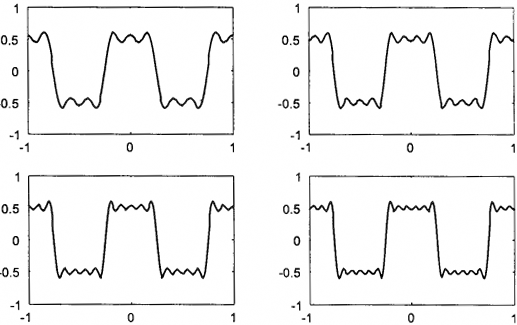
\includegraphics[scale=1]{gibbs}
\caption{Промежуточные стадии суммирования ряда Фурье для меандра}
\label{img:gibbs}
\end{figure}

\subsubsection{Преобразование Фурье}

Спектральный анализ -- 1 из способов обработки сигналов, который позволяет охарактеризовать частотный состав измеряемого сигнала.\linebreak Преобразование Фурье считается математической основой, которая связывает временной либо пространственный сигнал (или же некую модель данного сигнала) с его представлением в частотной области.

Для спектрального представления непериодических (импульсных)\linebreak сигналов $s\left(t\right)$, данных на конечном промежутке ($t_1$, $t_2$) (Рис.~\ref{img:f_trans}), конкретно воспользоваться рядом Фурье невозможно. Для гармонического разложения сигнала в мыслях дополняют его такими же импульсными сигналами до периодического с каким-либо промежутком $T$ (Рис.~\ref{img:f_trans}), при всем этом наполняя промежутки нулевыми значениями.

\begin{figure}[H]
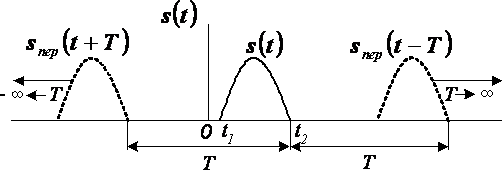
\includegraphics[width=\linewidth]{f_trans}
\caption{Импульсный сигнал $s\left( t\right)$ и его периодическое продолжение $s_{per}\left( t+kT\right)$.}\label{img:f_trans}
\end{figure}

С ростом периода следования импульсов гармоники расположены поближе друг к другу по частоте, а единый уровень спектральных составляющих становится все меньше. 

В пределе, при увеличении периода $T\rightarrow\infty$ все импульсы уйдут вправо и влево в бесконечность и периодическая последовательность вновь будет одиночным импульсом. Хотя взаимное соотношение меж уровнями гармоник останется постоянным и определяется все таким же интегралом (\ref{eq:fourier_koef}). В следствии этого при спектральном анализе непериодических сигналов формула для расчета коэффициентов комплексного ряда Фурье модифицируется следующим образом:

\begin{itemize}
\item частота перестает быть дискретно меняющейся и становится непрерывным параметров преобразования (то есть $k\omega$ в формуле ($\ref{eq:fourier_koef}$) заменяется на $\omega$);
\item удаляется множитель $1/T$;
\item результатом вычислений вместо нумерованных коэффициентов ряда $C_k$ является функция частоты $S_\omega$ -- \emph{спектральная функция} сигнала $s\left(t\right)$. Иногда ее называют \emph{спектральной плотностью}.
\end{itemize}

В результате перечисленных модификаций формула (\ref{eq:fourier_koef}) превращается в формулу \emph{прямого преобразования Фурье}:
\begin{equation}
\dot{S}\left(\omega\right)=\int_{-\infty}^\infty s\left(t\right)\mathrm{e}^{-\mathrm{j}\omega t}\mathrm{dt}.
\end{equation}

В формуле самого ряда Фурье (\ref{eq:fourier_series_exp}) суммирование заменяется интегрированием (и перед интегралом появляется деление на $2\pi$. Получающееся выражение называется \emph{обратным преобразованием Фурье}:
\begin{equation}
s\left(t\right)=\frac{1}{2\pi}\int_{-\infty}^{\infty}\dot{S}\left(\omega\right)\mathrm{e}^{\mathrm{j}\omega t}\mathrm{dw}.
\end{equation}

Чтобы преобразование Фурье было применимо, сигнал должен удовлетворять следующим требованиям:
\begin{itemize}
\item должны выполняться условия Дирихле;
\item сигнал должен быть \emph{абсолютно интегрируемым}:
\begin{equation}
\nonumber
\int_{-\infty}^{\infty}|s\left(t\right)|\mathrm{dt} < \infty.
\end{equation}
\end{itemize}

Модуль спектральной функции называется \emph{амплитудным спектром}, а ее аргумент -- \emph{фазовым диапазоном}.

Преобразование Фурье взаимно-однозначно, в следствии этого спектральная функция имеет столько-же информации, какое количество и исходный сигнал.

\subsubsection{Свойства преобразования Фурье}

Под свойствами преобразования Фурье предполагается взаимное соответствие трансформаций сигналов и их спектров.


Далее будем рассматривать два абстрактных сигнала, $f\left(t\right)$ и $g\left(t\right)$, и считать, что их спектральные функции равны $\dot{F}\left(\omega\right)$ и $\dot{G}\left(\omega\right)$, а встречающиеся параметры $\alpha$ и $\beta$ -- константы.

\begin{enumerate}
\item \textbf{Линейность}: если мы берем какую-то линейную комбинацию\linebreak функций, то преобразование Фурье этой комбинации будет такой же линейной комбинацией образов Фурье этих функций. Это свойство позволяет сводить сложные функции и их фурье-образы к более простым.
\begin{equation}
\nonumber
\text{Если }
s\left(t\right)=\alpha f\left(t\right)+\beta g\left(t\right)
\text{, то }
\dot{S}\left(\omega\right)=\alpha\dot{F}\left(t\right)+\beta\dot{G}\left(t\right).
\end{equation}

\item \textbf{Задержка}: независимость амплитудного спектра от сдвига сигнала по времени. Если мы подвинем функцию влево или вправо по оси x, то поменяется лишь ее фазовый спектр.
\begin{equation}
\nonumber
\text{Если }
s\left(t\right)=f\left(t-\tau\right)
\text{, то }
\dot{S}\left(\omega\right)=\dot{F}\left(\omega\right)\mathrm{e}^{-\mathrm{j}\omega\tau},
\end{equation}
где $\tau$ -- задержка.

\item \textbf{Перемена масштаба оси времени}: растяжение (сжатие) исходной функции по оси времени пропорционально сжимает (растягивает) ее фурье-образ по шкале частот. А именно, спектр сигнала конечной длительности постоянно бесконечно широк и напротив, диапазон конечной ширины всегда соответствует сигналу нелимитированной продолжительности. 

\begin{equation}
\nonumber
\text{Если }
s\left(t\right)=f\left(\alpha t\right)
\text{, то }
\dot{S}\left(\omega\right)=\frac{1}{|\alpha|}\dot{F}\left(\frac{\omega}{\alpha}\right), \alpha\neq 0.
\end{equation}

\item \textbf{Дифференцирование сигнала}: спектр производной получается путем умножения исходного сигнала на $j\omega$ -- оператор дифференцирования сигнала в частотной области. При дифференцировании низкие частоты ослабляются, а высокие усиливаются. Фазовый спектр сигнала сдвигается на $90^\circ$ для положительных частот и на $-90^\circ$ для отрицательных.
\begin{equation}
\text{Если }
s\left(t\right)=\frac{\mathrm{df}}{\mathrm{dt}}
\text{, то }
\dot{S}\left(\omega\right)=\mathrm{j}\omega\dot{F}\left(\omega\right).
\label{eq:diff_trans}
\end{equation}

\item \textbf{Интегрирование сигнала}: из (\ref{eq:diff_trans}) \emph{формально} следует, что спектр первообразной
\begin{equation}
\nonumber
\dot{S}\left(\omega\right)=\frac{\dot{F}\left(\omega\right)}{\mathrm{j}\omega}.
\end{equation}

Таким образом, множитель $1/(\mathrm{j}\omega)$ служит \emph{оператором интегрирования в частотной области}.

Однако формула выше справедлива лишь для сигналов, не содержащих постоянной составляющей, у которых
\begin{equation}
\nonumber
\dot{F}\left(0\right)=\int_{-\infty}^\infty f\left(t\right)\mathrm{dt}=0.
\end{equation}

В общем случае результат выглядит следующим образом
\begin{equation}
\nonumber
\dot{S}\left(\omega\right)=\frac{\dot{F}\left(\omega\right)}{\mathrm{j}\omega}+\pi\dot{F}\left(0\right)\delta\left(\omega\right).
\end{equation}

Наконец, интегрирование сигнала действует аналогично фильтру нижних частот, ослабляя высокочастотные спектральные составляющие входного сигнала.

\item \textbf{Спектр свертки сигналов}: по определению, свертка -- это математическая операция, примененная к двум функциям $f$ и $g$, порождающая третью функцию, которая иногда может рассматриваться как модифицированная версия одной из первоначальных:
\begin{equation}
\nonumber
s\left(t\right)=\left(f*g\right)\left(t\right)=\int_{-\infty}^\infty {f\left(t'\right)g\left(t-t'\right)\mathrm{dt'}}.
\end{equation}

Спектр свертки функций равен произведению их спектров:
\begin{equation}
\nonumber
\dot{S}\left(\omega\right)=\dot{F}\left(\omega\right)\dot{G}\left(\omega\right).
\end{equation}

Операция свертки коммутативна.

\item \textbf{Спектр произведения сигналов} представляет собой свертку\linebreak спектров, умноженную на $1/(2\pi )$:
\begin{equation}
\nonumber
\text{Если }
s\left(t\right)=f\left(t\right)g\left(t\right)
\text{, то }
\dot{S}\left(\omega\right)=\frac{1}{2\pi}\int_{-\infty}^\infty {\dot{F}\left(\tau\right)\dot{F}\left(t-\tau\right)\mathrm{d\tau}}.
\end{equation}

\item \textbf{Умножение сигнала на гармоническую функцию}: умножим исходный сигнал, спектр которого нам известен, на гармоническую функцию:
\begin{equation}
\nonumber
s\left(t\right)=f\left(t\right)\cos\left(\omega_0 t+\phi_0\right),
\end{equation}
тогда получим спектр сигнала:
\begin{equation}
\dot{S}\left(\omega\right)=\frac{1}{2}\mathrm{e}^{\mathrm{j}\phi_0}\dot{F}\left(\omega-\omega_0\right)+\frac{1}{2}\mathrm{e}^{-\mathrm{j}\phi_0}\dot{F}\left(\omega+\omega_0\right).
\end{equation}

Спектр "<раздвоился"> -- распался на два слагаемых вдвое меньшего уровня (множитель $1/2$), смещенных на $\omega_0$ вправо ($\omega-\omega_0$) и влево ($\omega+\omega_0$) по оси частот.
\end{enumerate}

\subsubsection{Корреляционный анализ сигналов}

Одним из традиционных способов исследования структуры сигналов считается корреляционный анализ, который находит бессчетные использования в задачах, связанных с передачей информации, радарным обнаружением, системами управления и т.д.. Ковариационные (корреляционные) функции дозволяют различные варианты интерпретации. С одной стороны, они позволяют выявлять степень сходства (линейной зависимости) 2-ух сигналов при варьировании сдвига по времени меж ними. В этом случае говорят о обоюдных ковариационных (взаимных корреляционных) функциях. С другой стороны, они применимы для изучения взаимосвязи значений одного и того же случайного процесса в разные моменты времени, что позволяет использовать терминологию автоковариационных (автокорреляционных) функций.

\textbf{Взаимная корреляционная функция}  (ВКФ; англ. -- cross-correla\-tion function, CCF) для двух сигналов $u\left(t\right)$ и $v\left(t\right)$:
\begin{equation}
\nonumber
\begin{split}
  w\left(t\right)&=u\left(t\right)\otimes v\left(t\right)\triangleq\int_{-\infty}^{\infty}{u^*\left(\tau\right)v\left(\tau +t\right)\mathrm{d\tau}}= \\
  &=\int_{-\infty}^{\infty}{u^*\left(\tau-t\right)v\left(\tau\right)\mathrm{d\tau}} \text{ [подстановка: $\tau\rightarrow\tau-t$]}
\end{split}
\end{equation}
где $u^*\left(t\right)$ -- комплексно-сопряженная функция к $u\left(t\right)$. Аргумент функции $w\left(t\right)$ называется задержкой и соответствует сдвигу фаз, который необходимо осуществить для одного сигнала ($v$) относительно другого ($u$), т.е. $t$ -- задержка $u$ относительно $v$.

ВКФ очень похожа на свертку двух сигналов:
\begin{align}
\nonumber
  u\left(t\right)\otimes v\left(t\right) &= \int_{-\infty}^{\infty}{u^*\left(\tau\right)v\left(\tau +t\right)\mathrm{d\tau}} & \text{[корреляция]} \\
  u\left(t\right)\ast v\left(t\right) &= \int_{-\infty}^{\infty}{u\left(\tau\right)v\left(t-\tau\right)\mathrm{d\tau}} & \text{[свертка]} \label{eq:def_conv}
\end{align}
Используя определение свертки (\ref{eq:def_conv}) при подстановке $\tau\rightarrow\tau-t$, можно перейти к ВКФ. Пусть $x\left(t\right)=u^*\left(-t\right)$, тогда
\begin{align*}
\nonumber
  x\left(t\right)\ast v\left(t\right)\triangleq \int_{-\infty}^{\infty}{x\left(t-\tau\right)v\left(\tau\right)\mathrm{d\tau}} = \\
  = \int_{-\infty}^{\infty}{u^*\left(\tau-t\right)v\left(\tau\right)\mathrm{d\tau}} = u\left(t\right)\otimes v\left(t\right).
\end{align*}
Преобразование Фурье сигнала $x\left(t\right)$:
\begin{align*}
  \dot{X}\left(\omega\right)=\int_{-\infty}^{\infty}{x\left(t\right)\mathrm{e}^{-\mathrm{j}\omega t}\mathrm{dt}}&=\int_{-\infty}^{\infty}{u^*\left(-t\right)\mathrm{e}^{-\mathrm{j}\omega t}\mathrm{dt}}=\int_{-\infty}^{\infty}{u^*\left(t\right)\mathrm{e}^{\mathrm{j}\omega t}\mathrm{dt}} = \\
  &=\left(\int_{-\infty}^{\infty}{u\left(t\right)\mathrm{e}^{\mathrm{j}\omega t}\mathrm{dt}}\right)^*=\dot{U}^*\left(\omega\right).
\end{align*}
Таким образом, $w(t)=x(t)\ast v(t)\Rightarrow \dot{W}(\omega)=\dot{X}(\omega)\dot{V}(\omega)=\dot{U}^*(\omega)\dot{V}(\omega)$, т.к. спектр свертки равен произведению их спектров. В итоге можно записать похожую теорему взаимной корреляции:
\begin{equation}
w(t)=u(t)\otimes v(t)=u^*(-t)\ast v(t)\Leftrightarrow \dot{W}(\omega)=\dot{U}^*(\omega)\dot{V}(\omega). \label{eq:def_cross_corr}
\end{equation}
В отличие от свертки, корреляция не ассоциативна и не коммуникативна:
\begin{equation}
\nonumber
  v(t)\otimes u(t)=v^*(-t)\ast u(t)=u(t)\ast v^*(-t)=w^*(-t).
\end{equation}
Указанная ранее ВКФ используется для сигналов с конечной энергией (energy signals), т.е. для непериодических. ВКФ для двух сигналов с бесконечной энергией (power signals), т.е. для периодических, вычисляется так:
\begin{equation}
\nonumber
  \lim_{T\rightarrow\infty}\frac{1}{T}\int_{-T/2}^{T/2}{u^*(\tau)v(\tau+t)\mathrm{d\tau}},
\end{equation}
однако если $u$ и $v$ -- периодические с периодом $T$, то формула лишается предела.

Известно, что $|w(t)|\leq\sqrt{E_uE_v}$ для любых $t$, где $E_u$ и $E_v$ -- энергии соответствующих сигналов, вычисляемые по формуле:
\begin{equation}
\nonumber
  E=\int_{-\infty}^{\infty}{|s(t)|}^2\mathrm{dt}.
\end{equation}
Можно определить нормализованную ВКФ:
\begin{equation}
\nonumber
  z(t)=\frac{u(t)\otimes v(t)}{\sqrt{E_uE_v}},
\end{equation}
с помощью которой можно измерять взаимную корреляцию в фиксированном масштабе между $-1$ и $+1$. Величина $z(t)$ известна как \emph{коэффициент взаимной корреляции} и имеет следующие параметры:
\begin{enumerate}
\item $|z(t)|\leq 1$ для всех $t$;
\item $|z(t_0)|=1\Leftrightarrow v(\tau)=\alpha u(\tau -t)$, $\alpha$ -- константа.
\end{enumerate}
Иными словами, значение $+1$ указывает на полное совпадение сигналов, $0$ -- отсутствие корреляции, а $-1$ -- $100\%$-ная корреляция в противоположном смысле, например, как для сигналов в противофазе.

ВКФ обладает еще несколькими свойствами:
\begin{itemize}
\item $w_{uv}(-t)=w_{vu}(t)$, то есть изменение знака $t$ равносильно взаимной перестановке сигналов;
\item с ростом абсолютного значения $t$ ВКФ сигналов с конечной энергией затухает: $\lim_{|t|\rightarrow\infty}w(t)=0$;
\item значение ВКФ при $t=0$ ничем не выделяется, а максимум может быть расположен в любом месте оси $t$.
\end{itemize}

\textbf{Автокорреляция} -- это нахождение корреляции одного сигнала с самим собой. Автокорреляция является частным случаем взаимной корреляции и определяется формулой (для непериодических сигналов):
\begin{equation}
\nonumber
w(t)=u(t)\otimes u(t)=\int_{-\infty}^{\infty}{u^*(\tau\pm t)u(\tau)\mathrm{d\tau}}.
\end{equation}
Автокорреляция при нулевой задержке для непериодического сигнала равно его энергии:
\begin{align}
\nonumber
  w(0)=\int_{-\infty}^{\infty}{u^*(\tau-0)u(\tau)\mathrm{d\tau}}=\int_{-\infty}^{\infty}{|u(\tau)|^2\mathrm{d\tau}}=E_u.
\end{align}
Нормализованная автокорреляция: $z(t)=\frac{u(t)\otimes u(t)}{E_u}$ удовлетворяет свойствам $z(0)=1$ и $|z(t)|\leq 1$ для любого $t$.
По теореме взаимной корреляции~(\ref{eq:def_cross_corr}),
\begin{equation}
\nonumber
  w(t)=u(t)\otimes u(t) \Leftrightarrow \dot{W}(\omega)=\dot{U}^*(\omega)\dot{U}(\omega)=|\dot{U}(\omega)|^2,
\end{equation}
т.е. преобразование Фурье автокорреляциионной функции есть спект\-ральная плотность мощности (energy spectrum).

Автокорреляция для периодических сигналов с периодом $T$ определяется:
\begin{equation}
\nonumber
w(t)=\frac{1}{T}\int_{-T/2}^{T/2}{u(\tau)u(\tau-t)\mathrm{d\tau}},
\end{equation}
тогда при задержке $t=0$ получим среднюю мощность сигнала $P_u$:
\begin{equation}
w(0)=\frac{1}{T}\int_{T}{u^2(\tau)\mathrm{d\tau}}=P_u.
\end{equation}

Значение корреляционной функции при $t=0$ для обоих типов сигналов является максимально возможным: $|w(t)|\leq w(0)$. Также имеется свойство четности: $w(t)=w(-t)$.

Расчет корреляции можно ускорить, используя теорему о корреляции, которая обычно формулируется следующим образом:
\begin{equation}
w(t)=\dot{F_D}^{-1}\left[\dot{U}^*(\omega)\dot{V}(\omega)\right],
\end{equation}
где $\dot{F_D}^{-1}$ обозначает обратное преобразование Фурье. Данный подход требует двух дискретных преобразований Фурье (ДПФ) и одного обратного ДПФ, что легче всего сделать, используя алгоритм БПФ. Если число членов в последовательностях достаточно велико, данный метод БПФ дает результат быстрее, чем непосредственный расчет взаимной корреляции.

\subsection{Ход работы}

\subsubsection{Прямоугольный импульс}

Единичный прямоугольный импульс, центрированный относительно начала отсчета времени, с амплитудой $A$ и длительностью $T$ можно представить выражением:
\begin{equation}
\nonumber
s\left(t\right)=
  \begin{cases}
    A, &|t| \leq T/2, \\
    0, &|t| > T/2.
  \end{cases}
\end{equation}

Преобразование Фурье прямоугольного импульса:
\begin{equation}
\begin{split}
\nonumber
\dot{S}\left(\omega\right)&=\int_{-T/2}^{T/2}{A\mathrm{e}^{-\mathrm{j}\omega t}\mathrm{dt}}=\frac{2A}{\omega}\sin\left(\frac{\omega T}{2}\right)=AT\frac{\sin\left(\omega T/2\right)}{\omega T/2}= \\
&= AT\cdot\mathrm{sinc}\left(\omega T/2\right).
\end{split}
\end{equation}

Пик амплитудного спектра расположен в нуле ($\omega=0$) со значением, равным $AT$. Нули спектра встречаются при значениях, кратных $2\pi/T$, т.е. $(\pm 2\pi/T, \pm 4\pi/T, \pm 8\pi/T, \ldots)$.

Сформировал прямоугольный импульс с единичной амплитудой и длительностью $T=0.2$ с помощью встроенной функции -- $rectpulse(t,w)$:
\begin{verbatim}
fs = 500; % частота дискретизации
T = 0.2; % длительность прямоугольного импульса

t = -0.5:1/fs:0.5; % отсчеты времени
 
x = rectpuls(t, T); % генерация импульса
\end{verbatim}

Функция $FFT$ в Matlab используется для вычисления дискретного преобразования Фурье ($DFT$). Результат БПФ изображен на Рис.~\ref{img:sp_rect_pulse}. С приведенного графика следует, что пик амплитуды действительно находится при $\omega=0$ ($f=0$) со значением $AT=1\times 0.2=0.2$. Нули спектра расположены при $f=(\pm 1/T=5, \pm 2/T=10, \pm 3/T=15,\ldots)$, как и ожидалось.
\begin{verbatim}
L=length(x);
NFFT = 500; % количество линий Фурье спектра
% FFT вместе с FFTshift для отрицательных и полож. частот
X = fftshift(fft(x,NFFT));
f = fs*(-NFFT/2:NFFT/2-1)/NFFT; % вектор частот

plot(t, x, 'k');
plot(f,abs(X)/(L), 'r');
plot(f, atan2(imag(X),real(X))*180/pi);
\end{verbatim}
\begin{figure}[H]
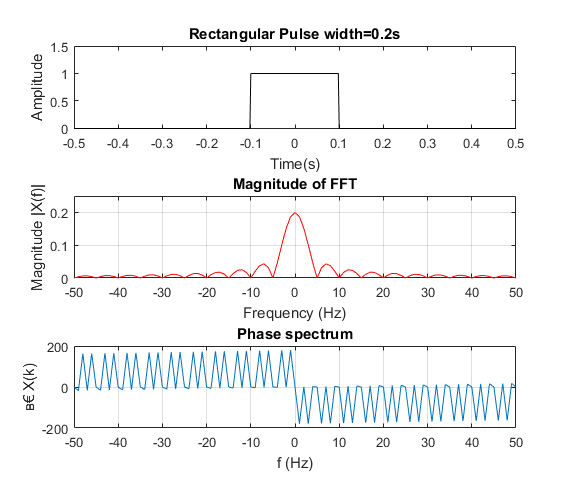
\includegraphics[width=\linewidth]{sp_rect_pulse}
\caption{Прямоугольный импульс и его амплитудный и фазовый спектры.}
\label{img:sp_rect_pulse}
\end{figure}

\subsubsection{Симметричный треугольный импульс}

Симметричный треугольный импульс, центрированный относительно начала отсчета времени, с амплитудой $A$ и длительностью $\tau=2\cdot T$, где $T$~-- \emph{эффективная ширина спектра}, можно представить выражением:
\begin{equation}
\nonumber
s\left(t\right)=
  \begin{cases}
    A\left(1-\frac{|t|}{T}\right), &|t| \leq T, \\
    0, &|t| > T.
  \end{cases}
\end{equation}

Вычислил преобразование Фурье треугольного импульса:
\begin{equation}
\nonumber
\dot{S}\left(\omega\right)=\int_{-T}^T{A\left(1-\frac{|t|}{T}\right)\mathrm{e}^{-\mathrm{j}\omega t}\mathrm{dt}}=AT\frac{\sin^2\left(\omega T/2\right)}{\left(\omega T/2\right)^2}.
\end{equation}

Сформировал треугольный импульс с амплитудой $A=2$ и длительностью $\tau=2*T=2*0.1=0.2$ с помощью встроенной функции -- $tripuls(t,w)$:
\begin{verbatim}
fs = 500; % частота дискретизации
T = 0.1; % ширина треугольного импульса
t = -0.5:1/fs:0.5; % отсчеты времени
A = 2; % амплитуда
% домножаем T на 2, чтобы получить длительность импульса
x = A*tripuls(t, 2*T); % генерация импульса
\end{verbatim}

Далее построил график амплитудного спектра так же, как это было сделано для прямоугольного импульса. Спектр приведен на Рис.~\ref{img:sp_tri_pulse}. Видно, что пик находится при $\omega=0$ ($f=0$) со значением амплитуды $AT=2\times 0.1=0.2$. Нули спектра расположены при значениях, кратных $pi/T$ (или, если использовать не круговую частоту, а обычную -- $f=(\pm 1/T=10, \pm 2/T=20, \pm 3/T=30,\ldots)$).
\begin{figure}[H]
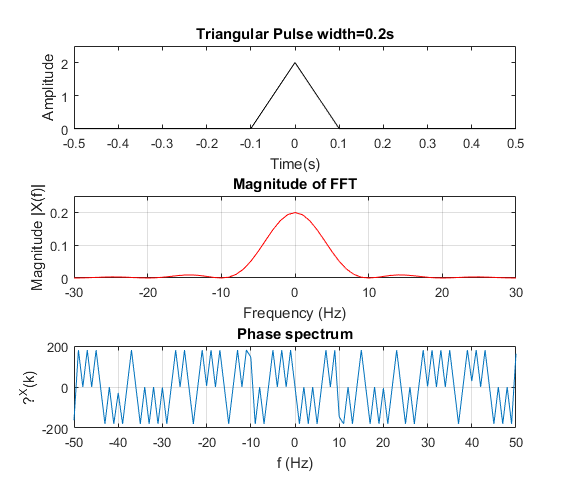
\includegraphics[width=\linewidth]{sp_tri_pulse}
\caption{Треугольный импульс и его амплитудный и фазовый спектры.}
\label{img:sp_tri_pulse}
\end{figure}

\subsubsection{Гармонический сигнал}


Одним из наиболее часто используемых типов детерминированных периодических сигналов является гармоническое колебание, описываемое уравнением $s\left(t\right)=A\sin\left(\omega_0t+\phi_0\right)$, где $A$ -- амплитуда, $\omega_0$ -- частота (круговая), $\phi_0$ -- начальная фаза. Величина $\left(\omega_0 t+\phi_0\right)$ определяет полную фазу сигнала. Таким образом, гармоническое колебание полностью характеризуется тремя параметрами: частотой (или периодом), амплитудой и фазой.

Синтезировал в Matlab гармонический сигнал, повторяющийся 5 периодов, с частотой $10$ Гц, амплитудой $1.5$ и фазой $\pi/4$:
\begin{verbatim}
f = 10; % частота гарм. сигнала
Fs = 100; % частота дискретизации
Ph = pi/4; % фазовый сдвиг (рад)
nCyl = 5; % чтобы сгенерировать 5 периодов
A = 1.5; % амплитуда
 
t = 0:1/Fs:nCyl*1/f; % дискр. отсчеты времени

x = A*sin(2*pi*f*t + Ph); % синтез сигнала
\end{verbatim}

Рассчитал спектральную функцию гармонического сигнала:
\begin{equation}
\nonumber
\begin{split}
  \dot{S}\left(\omega\right)&=\int_{-\infty}^{\infty}{A\cos\left(\omega_0 t+\phi_0\right)\mathrm{e}^{-\mathrm{j}\omega t}\mathrm{dt}}=\int_{-\infty}^{\infty}{A\frac{\mathrm{e}^{\mathrm{j}\omega t+\mathrm{j}\phi_0}+\mathrm{e}^{-\mathrm{j}\omega_0 t-\mathrm{j}\phi_0}}{2}\mathrm{e}^{-\mathrm{j}\omega t}\mathrm{dt}}=\\
  &=\int_{-\infty}^{\infty}{\frac{A}{2}\mathrm{e}^{\mathrm{j}\phi_0}\mathrm{e}^{-\mathrm{j}\left(\omega -\omega_0\right)t}\mathrm{dt}}+\int_{-\infty}^{\infty}{\frac{A}{2}\mathrm{e}^{-\mathrm{j}\phi_0}\mathrm{e}^{-\mathrm{j}\left(\omega+\omega_0\right)t}\mathrm{dt}}=\\
  &=A\pi\mathrm{e}^{\mathrm{j}\phi_0}\delta\left(\omega-\omega_0\right)+A\pi\mathrm{e}^{-\mathrm{j}\phi_0}\delta\left(\omega+\omega_0\right).
\end{split}
\end{equation}

Результат, как видно из получившегося выражения, представляет собой пару дельта-функций, расположенных на частотах $\pm\omega_0$. Множители при них отражают амплитуду и начальную фазу гармонического сигнала. Для сгенерированного сигнала спектр должен содержать две гармоники на частотах $\pm10$ Гц с амплитудой $A/2=1.5/2=0.75$. Проверил это, построив амплитудный и фазовый спектры сигнала (Рис.~\ref{img:sp_sin}):
\begin{verbatim}
NFFT = 550;	% % число линий Фурье спектра
X = fftshift(fft(x,NFFT)); % получаем спектр
fVals = Fs*(-NFFT/2:NFFT/2-1)/NFFT;	% вектор частот	 

plot(t, x, 'k');
plot(fVals, abs(X)/length(x), 'r');	 	 
plot(fVals, atan2(imag(X),real(X))*180/pi);
\end{verbatim}
\begin{figure}[H]
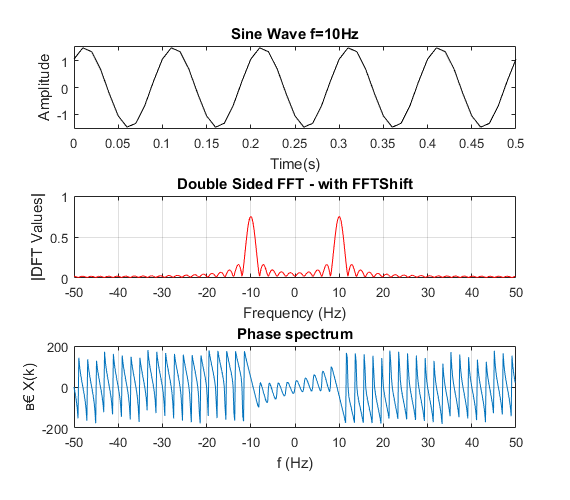
\includegraphics[width=\linewidth]{sp_sin}
\caption{Гармонический сигнал и его амплитудный и фазовый спектры.}
\label{img:sp_sin}
\end{figure}

\subsubsection{Сигнал с меняющейся частотой (chirp)}

Получил сигнал с частотой изменяющейся во времени с помощью функции Matlab $chirp$. Частота chirp сигнала может варьироваться от низких до высоких частот (up-chirp) или от высоких к низким (low-chirp).

Chirp сигналы встречаются всюду, например, частота движения маятника меняется со временем. Доплеровский эффект, радары, сонары, обработка изображений -- и там встречаются chirp сигналы.

Линейный chirp сигнал меняет частоту от низкой до высокой или наоборот линейно во времени. Чтобы сгенерировать такой сигнал, можно модифицировать уравнение гармонического сигнала и воспользоваться им:
\begin{equation}
\begin{split}
s\left(t\right)&=A\cos\left(2\pi f\left(t\right)t+\phi_0\right), \\
\text{где }
f\left(t\right)&=\frac{k}{2}t+f_0 \text{ и }
k=\frac{f_1-f_0}{t_1-t_0},
\end{split}
\end{equation}
причем $f_0,f_1$ -- начальная и конечная частоты; $t_0, t_1$ -- первый и последний временной отсчет; $\phi_0$ -- начальная фаза; $A$ -- амплитуда.

Я для создания сигнала воспользовался встроенной в Matlab функцией $chirp$.
\begin{verbatim}
fs = 500; % частота дискретизации
t = 0:1/fs:1; % отсчеты времени
 
f0 = 1; % начальная частота chirp
f1 = 25; % частота chirp при t = 1 (в конце)
x = chirp(t, f0, 1, f1);
\end{verbatim}

График полученного сигнала представлен на Рис.~\ref{img:sp_chirp}. Видно, как частота колебания сигнала меняется от низких значений до высоких линейно во времени. Затем построил амплитудный и фазовый спектры синтезированного chirp сигнала.
\begin{figure}[H]
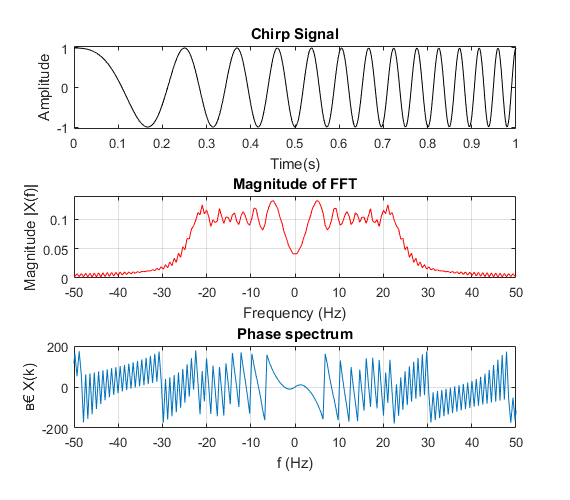
\includegraphics[width=\linewidth]{sp_chirp}
\caption{Chirp сигнал и его амплитудный и фазовый спектры.}
\label{img:sp_chirp}
\end{figure}

\subsubsection{Поиск синхропосылки с помощью xcorr}

Представил сигнал [0001010111000010] в виде последовательности прямоугольных импульсов с частотой $1600$\,Гц (период $T=1/Fs$) и коэффициентом заполнения, равным $100\%$. Для этого увеличил число отсчетов в сигнале в $100$ раз с помощью функции $bld\_signal$:
\begin{verbatim}
function s = bld_signal(x, scale);
s = zeros(1, numel(x)*scale);
k = 1;
for i=1:numel(s)
  if(i/k > scale)
    k = k + 1;
  end
  s(i) = x(k);
end
\end{verbatim}
После такого преобразования сигнал будет иметь $1600$ отсчетов. Проделал то же с сигналом синхропосылки [101]:
\begin{verbatim}
r = [0 0 0 1 0 1 0 1 1 1 0 0 0 0 1 0]; % сигнал
m = [1 0 1]; % синхропосылка (шаблон)
scale = 100; % во сколько "растянуть" сигналы
% e.g. для [1 0], scale=2: [1 1 0 0];
r = bld_signal(r, scale);
m = bld_signal(m, scale);
% пусть частота дискретизации соответствует числу отсчетов
Fs = (numel(r)-1);
\end{verbatim}
Графики получившихся сигналов приведены на Рис.~\ref{img:xcorr_tsa}.
\begin{figure}[H]
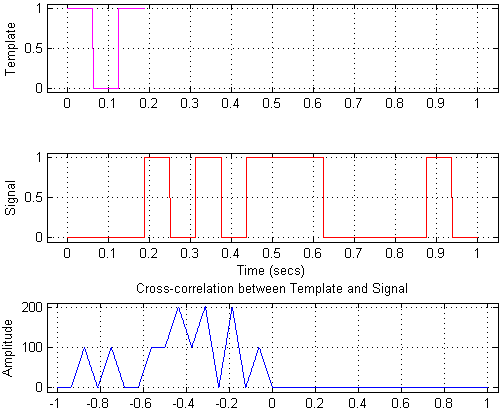
\includegraphics[width=\linewidth]{xcorr_tsa}
\caption{Синхропосылка и сигнал, а также график их корреляции.}
\label{img:xcorr_tsa}
\end{figure}

Рассчитал коэффициенты корреляции (вектор $C$) с помощью встроенной в Matlab функции $xcorr$:
\begin{verbatim}
[C, lag] = xcorr(m, r); % вычисление корреляции
\end{verbatim}
На выходе получил вектор задержек $lag$ для каждого коэффициента из $C$. И уже возможно вычислить начало синхропосылки. Чтобы достичь желаемого результата необходимо обнаружить пик в $C$ (см. Рис.~\ref{img:xcorr_tsa}). Пиков может быть несколько, хотя необходим последний, т.к. предыдущие имеют все шансы указывать не на синхропосылку, а на сигнал с информацией после нее. В следствии этого поначалу я определил значение максимума в $C$, а потом вычислил позицию последнего встретившегося этого элемента с погрешностью в $5\%$ -- в следствии тестов выяснилось, что значения пиков могут незначительно отличаться, а функция $max$ находит наибольший из них, что приводит к некорректному результату. Теперь осталось определить задержку:
\begin{verbatim}
>> Z = max(abs(C)); % поиск наибольшего коэффициента
>> I = find(abs(C-Z) < Z*0.05, 1, 'last');
>> SampleDiff = lag(I) % выводим значение задержки
>> SampleDiff =
     -295
>> timediff = SampleDiff/Fs % переводим в единицы времени
>> timediff =
     -0.1845
\end{verbatim}
Выразил задержку как число отсчетов и в единицах времени. Последний пик на графике взаимной корреляции означает, что синхропосылка появляется в сигнале после $0.1845$. Иными словами, синхропосылка опережает сигнал на $295$ отсчетов, на что указывает $SampleDiff$. Эта информация пригодится для выравнивания сигналов друг относительно друга:
\begin{verbatim}
if(SampleDiff == 0) SampleDiff = 1; end; % r(0:end) - нельзя
r_al = r(abs(SampleDiff):end); % выравнивание сигнала
\end{verbatim}
Результат представлен на Рис.~\ref{img:xcorr_ts}.
\begin{figure}[H]
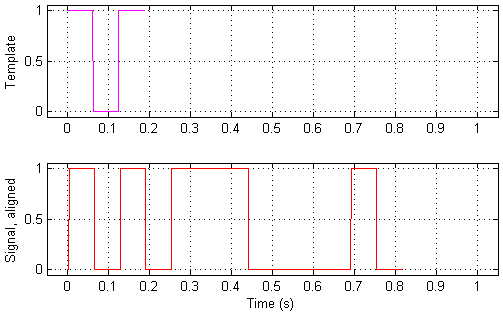
\includegraphics[width=\linewidth]{xcorr_ts}
\caption{Синхропосылка и выравненный сигнал.}
\label{img:xcorr_ts}
\end{figure}

Теперь несложно определить пакет данных:
\begin{verbatim}
lm = 8; % длина пакета данных
p = zeros(1, lm); % выделение памяти под пакет с данными
for i=0:lm-1
  % смотрим значение сигнала в середине импульса и
  p(i+1) = r_al(350+i*scale); % пропускаем 3 имп. синхропосылки
end
\end{verbatim}
В результате $p$ равен [01110000].

\subsubsection{Поиск синхропосылки с помощью быстрой корреляции}

Для данной задачи синхропосылка и сигнал были преобразованы так же, как и в предыдущем случае. Их графики можно посмотреть на Рис.~\ref{img:xcorr_tsa}.

Основное отличие в расчете коэффициентов корреляции. В этот раз сначала сигналы подвергаются быстрому преобразованию Фурье (дискретному), затем перемножаются, после чего произведение передается в функцию обратного дискретного преобразования Фурье:
\begin{verbatim}
C = ifft(fft(fliplr(r), 2*Fs).*fft(fliplr(m), 2*Fs), 2*Fs);
lag = [-Fs:Fs-1]; 
\end{verbatim}
Отмечу, что синхропосылка и сигнал были представлены в обратном порядке ($fliplr$). Это нужно для того, чтобы график корреляции был идентичен таковому на Рис.~\ref{img:xcorr_tsa} и чтобы можно было выполнять те же дальнейшие действия. Также был сформирован вектор задержек.

Оставшиеся шаги полностью совпадают с тем, что проделано в случае с использованием $xcorr$: нашел задержку как число отсчетов, выровнял сигналы, показал график, определил посылку.

Продемонстрирую работу быстрой корреляции на примере с сигналом [0101010111000010]:
\begin{figure}[H]
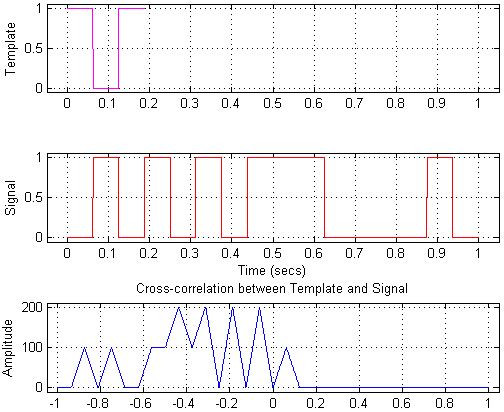
\includegraphics[width=\linewidth]{fcorr_tsa}
\caption{Синхропосылка и сигнал, а также график их корреляции.}
\label{img:fcorr_tsa}
\end{figure}
\begin{figure}[H]
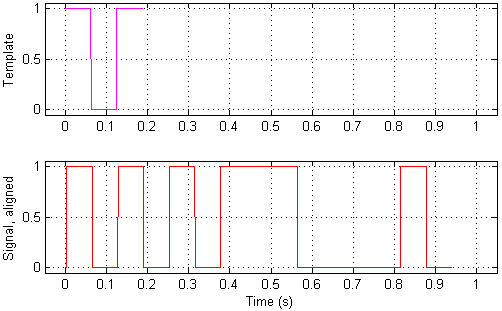
\includegraphics[width=\linewidth]{fcorr_ts}
\caption{Синхропосылка и выравненный сигнал.}
\label{img:fcorr_ts}
\end{figure}

В результате получена посылка: [01011100].

\subsubsection{Сравнение xcorr с быстрой корреляцией}
Для сравнения воспользовался функциями Matlab $tic$ и $toc$: первая используется в том месте, откуда следует начать отсчет времени, последняя~-- там, где нужно завершить счет и вывести результат.

Сравниваться будет только время формирования векторов коэффициентов корреляции и задержек для одинаковых сигналов.
\begin{itemize}
\item $xcorr$:
\begin{verbatim}
tic;
[C, lag] = xcorr(m, r);
toc
\end{verbatim}
\item быстрая корреляция
\begin{verbatim}
tic;
C=ifft(fft(fliplr(r),2*Fs).*fft(fliplr(m),2*Fs),2*Fs);
lag = [-Fs:Fs-1]; 
toc
\end{verbatim} 
\end{itemize}

В результате трех измерений каждого алгоритма установлено, что быстрая корреляция работает на $0.072$\,с быстрее, чем $xcorr$: $0.016$\,с против $0.088$\,с.

\subsection{Вывод}

Не считая естественного представления сигналов во временной области в анализе сигналов и систем обширно осуществляется частотное представление.

Пускай имется сигнал в виде комплекта отсчетов его амплитуд, производимых с некоторой частотой дискретизации. В этом виде удобно хранить сигнал и преобразовывать его обратно в непрерывный. Дабы иметь возможность обрабатывать сигнал, к примеру, определить степень сходства имеющегося сигнала с иным, потребуется преобразование представления сигнала в виде отсчетов в его частотный диапазон. Это осуществляется при помощи прямого (дискретного) преобразования Фурье. После этого преобразования сигнал будет представлен в виде коэффициентов, сообразных амплитудам и фазам частот, составляющих данный сигнал. Тогда возможно использовать такие операции обработки сигнала, как "<фильтр нижних частот"> либо "<фильтр верхних частот">, которые "<вырезают"> из сигнала все частоты выше или же ниже какой-либо заданной при помощи обнуления коэффициентов, соответствующие частотам, которые нужно убрать.

Круг областей применения преобразования Фурье существенно шире: обработка растровых изображений, телекоммуникации, исследование и измерение сигналов, радиолокация и так далее Образцом применения преобразования имеет возможность служить передача данных в цифровой форме по аналоговым линиям телефонной сети (модем). Для передачи данных в цифровой форме, они поначалу преобразуются в некоторый набор частот и передаются по линиям передач, а затем, на приемной стороне производится обратное преобразование и восстанавливаются начальные данные. 

Корреляционный анализ дозволяет решить часто образующуюся задачу обнаружения 1-го сигнала в другом. В основу корреляционного анализа положено вычисление корреляции, то есть
числового значения, описывающего меру связи сигналов на рассматриваемом временном промежутке. 

\end{document}